\documentclass[11pt]{article}
\usepackage[a4paper,portrait]{geometry}
\usepackage{graphicx}
\usepackage{fullpage}

\begin{document}
\title{\vspace{-1in}ARMv8 Project - Checkpoint 1}
\author {Gleb Koval, Mehmet Kaan Nur, Eren Geridonmez, Ali Kilic}
\date {7th June 2024}
\maketitle

\section{Group Organization}
\subsection{Separation of work} 

    Before we started the project, we separated the work so that each member of group can work on a part of the project. Gleb worked on the input/output processing function and single data instructions, Mehmet worked on register based data processing instructions, Eren worked on immediate value based data processing instructions, and Ali worked on branch instructions.
    
    We pushed commits into different Git branches for each type of instruction, which enabled us to ensure the master branch always had the finalized versions. Each teammate reviewed the merge requests before we merged them into the master branch.

    We always gave importance to communication to make each group member stay informed about the new updates in the code. We made sure to meet regularly to peer-program and review each other's code.

\subsection{Future improvements}

    Currently, code style is a bit inconsistent across the different commits. We could aim to fix this by forcing the use of a formatter on everyone's text editors - for example, the formatter from the C/C++ for VScode extension.


%**********************************************%
\section{Implementation of Emulator}
\subsection{Structure}

\includegraphics[width=\textwidth]{incgraph_emulate.eps}
This graph shows how the files in our project connect to each other. All files declare local types and static functions \textit{only} in the \verb|.c| file, and the rest in their respective header file.

\begin{itemize}
    
    \item \verb|emulate.c| contains the \verb|main| function for the emulator. Handles CLI arguments and opening/closing required input and output files.

    \item \verb|emulator.c| contains the following helper functions:
    \begin{itemize}
        \item \verb|make_emulstate| initialises the emulator state (memory, registers, state flags).
        \item \verb|fprint_emulstate| prints the emulator state into a text file.
        \item \verb|emulstep| executes a single instruction step. We check the \verb|op0| to determine the type of instruction and then run the function that will execute it. If we come across an unknown instruction or a halt instruction, we stop the program.
        \item \verb|get_reg| and \verb|set_reg| gets and sets register values in an \verb|emulstate| while correcting for 32/64-bit mode, ZR register, and out-of-range values.
        \item \verb|load_mem| and \verb|store_mem| loads and stores 32/64-bit values from/to the memory array in an \verb|emulstate|.
        \item \verb|get_value| gets a portion of a \verb|unsigned long| using an offset and bit length.
        \item \verb|sf_checker| applies a \verb|0xFFFFFFFF| mask to a \verb|unsigned long long| in 32-bit mode.
    \end{itemize}

    \item \verb|instr_branch.c| contains the functions that compute the branch instructions  and modifying the \verb|PC| according to the type (Unconditional, Register, Conditional) and the content of the instructions.  

    This file utilizes \verb|sign_extend_64bit| function which extends the sign of a long long value, provided the sign bit position.

    \item \verb|instr_dpimm.c| contains the functions that computes the immediate value based arithmetic (add, adds, sub, subs) and wide move (movn, movz, movk) instructions. Computes the shifted value of \verb|imm12| according to \verb|sh|, and performs the operation on the immediate value and a register value, saving the result to the \verb|rd| register.

    This file utilizes \verb|set_pstate_flags| function which sets the condition flags, provided the previous state, bit-width, register values, and operation type.

    \item \verb|instr_dpreg.c| contains the function that computes the register based arithmetic (add, adds, sub, subs), bit-logic (and, bic, orr, orn, eor, eon, ands, bics), and multiply (madd, msub) instructions. Computes the shifted version of \verb|rm| register according to \verb|opr|, and performs the required operation with \verb|rn| and shifted \verb|rm| registers, saving the output to the \verb|rd| register.

    \item \verb|instr_sdt.c| contains the function that computes the single data transfer instructions, by first calculating the memory address and then applying the load/store.
    
    This file utilizes a \verb|sign_extend| function which extends the sign of a long value, provided the sign bit position.

\end{itemize}

\subsection{Compatibility with Further Work}
The emulator and assembler are quite different programs, and so we don't expect to be able to reuse much between the two. The assembler will have a function very similar to \verb|get_value| from \verb|emulator.c|, but instead to \textit{set} a bit range in a \verb|unsigned long| that represents an instruction.

\subsection{Expected upcoming difficulties}
We believe that the most difficult part will be managing the compatibility of the assembler tokenizer with our emulator. Additionally, we need to understand the functionalities of Raspberry Pi to implement Part 3 correctly and efficiently.

\end{document}